\chapter{JavaScript}\label{cap:javaScript}
\epigraph{``\textit{A vida vai ficando cada vez mais dura perto do topo}''.}{Friedrich Nietzsche}

\lettrine[lines=4, lhang=0.1, lraise=0, loversize=0.2, findent=0.1em]{\textcolor{corAzulTema}{N}}{ESTE} Capítulo temos com objetivo aprender as construções básicas da linguagem de programação JavaScript, vastamente utilizada no desenvolvimento de aplicações Web.

\section{Introdução}

Chegamos a talvez à cereja do bolo, ou à cereja do livro ou então à cereja do desenvolvimento para Web: a linguagem de \textit{script} JavaScript. A primeira coisa que precisamos deixar claro é que Java e JavaScript são duas linguagens diferentes, com sintaxe baseada em C e com construções similares, mas o comum entre as duas para por aqui. A linguagem JavaScript não é uma linguagem orientada a objetos, mas sim baseada em protótipos. Nesse tipo de linguagem não existem classes, mas apenas objetos. Novos objetos são criados a partir de cópias de objetos existentes. O JavaScript moderno, baseado no padrão ECMAScript, possui algumas construções que lembram a orientação a objetos como classes e herança de entre classes, mas tudo isso é \textit{syntax sugar} para simplificar coisas que já existiam anteriormente. Outras construções também são suportadas na linguagem como as funções de primeira classe etc.

Neste Capítulo não entraremos em detalhes sobre a história da linguagem e da sua evolução, mas sim no que eu acho útil e fundamental para que possamos começar a usar a linguagem. Iremos ver uma visão geral da linguagem como declaração de variáveis, manipulação do \textit{Document Object Model} (DOM) e requisições assíncronas. Durante o Capítulo serão apresentadas inúmeras caixas do tipo ``Saiba Mais'' com \textit{links} úteis. A maioria desses links serão da \textit{Mozilla Developer Network}\footnote{\url{https://developer.mozilla.org/}} (MDN), uma referência confiável e oficial da maioria, senão de todas, das tecnologias para Web. Sempre fornecerei os \textit{links} da versão em inglês do site, mas se quiser, você pode verificar a versão em português clicando no botão ``\textit{Change language}'' presente em todas as páginas do site. Sinceramente recomendo a leitura em inglês, pois o texto sempre estará completo, atualizado com a terminologia correta.

\begin{saibaMais}
    Quer conhecer um pouco mais da história e dos detalhes da linguagem JavaScript? Veja o \textit{link} \url{https://developer.mozilla.org/en-US/docs/Web/JavaScript}.
\end{saibaMais}

\begin{saibaMais}
    A referência da linguagem JavaScript pode ser acessada pelo \textit{link} \url{https://developer.mozilla.org/en-US/docs/Web/JavaScript/Reference}.
\end{saibaMais}

\begin{saibaMais}
    As documentações e referências das tecnologias e APIs usadas para o desenvolvimento para Web podem ser acessadas pelo \textit{link} \url{https://developer.mozilla.org/en-US/docs/Web/API}.
\end{saibaMais}

\begin{saibaMais}
    Caso deseje fazer um tutorial completo sobre a linguagem recomendo o tutorial da própria MDN, que é muito bom: \url{https://developer.mozilla.org/en-US/docs/Learn/JavaScript}.
\end{saibaMais}


Antes de começarmos a falar do JavaScript propriamente dito, vamos montar nosso palco, que é um projeto Java para Web. Neste Capítulo ainda faremos a construção dos projetos do zero, mas a partir do próximo focarei apenas nas novidades que serão apresentadas.

Vamos lá. Crie um projeto Java Web com o nome de ``ExemplosEmJavaScript'' da forma que tem feito até aqui. Os passos descritos a seguir são somente estruturais. Os respectivos códigos dos arquivos serão apresentados e explicados posteriormente. Sendo assim, no nó \destaque{\textit{Web Pages}} do projeto:

\begin{itemize}
    \item Remova o arquivo \texttt{index.html};
    \item Crie um JSP chamado \texttt{index.jsp};
    \item Crie uma pasta chamada \texttt{css};
    \item Crie uma pasta chamada \texttt{js} (JavaScript);
    \item Dentro da pasta \texttt{css} crie um arquivo CSS chamado \texttt{estilos.css};
    \item Dentro da pasta \texttt{js} crie 12 arquivos JavaScript, chamados \texttt{exemplo01.js}, \texttt{exemplo02.js}... \texttt{exemplo12.js};
    \item Em \destaque{\textit{Source Packages}} crie os pacotes \texttt{exemplosemjavascript.pojo} e\newline%
    \texttt{exemplosemjavascript.servlets};
    \item No pacote \texttt{exemplosemjavascript.pojo} crie uma classe chamada \texttt{Pessoa};
    \item No pacote \texttt{exemplosemjavascript.servlets} crie os Servlets \texttt{CalculaTabuadaServlet} e \texttt{ListagemPessoasServlet};
    \item Importe e insira no projeto a biblioteca \texttt{Jakarta EE Web 8 API};
    \item Clique com o botão direito do mouse no nó raiz do projeto e escolha o último item do menu de contexto, chamado \destaque{\textit{Properties}};
    \begin{itemize}
        \item Do lado esquerdo, em \destaque{\textit{Categories:}}, clique no item \destaque{CDNJS}, situado dentro do nó \destaque{\textit{JavaScript Libraries}};
        \item Do lado direito, clique no botão \destaque{\textit{Add}};
        \item No diálogo que abriu, intitulado \destaque{\textit{Add CDNJS Library}}, preencha o campo \destaque{\textit{Find:}} com ``\texttt{jquery}'' (sem as aspas) e clique em \destaque{\textit{Search}};
        \item Após a busca na \textit{Content Delivery Network} (CDN) a aparecerão diversos componentes na \textit{Graphical User Interface} (GUI). Em \destaque{\textit{Libraries:}} escolha \texttt{jquery}, provavelmente o primeiro item;
        \item Em \destaque{\textit{Files:}} marque a \textit{checkbox} na frente do item \texttt{jquery.min.js} e clique em \destaque{\textit{Add Library}} como na Figura~\ref{fig:cap07AddCDNJSLibrary};
        \FloatBarrier
        \begin{figure}[!htbp]
            \centering
            \caption{Adicionando uma biblioteca JavaScript}
            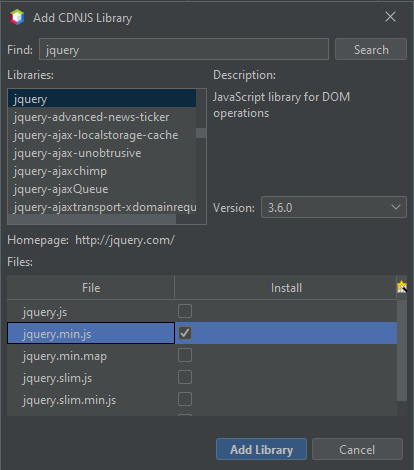
\includegraphics[scale=0.7]{imagens/cap07AddCDNJSLibrary}
            \\\textbf{Fonte:} Elaborada pelo autor
            \label{fig:cap07AddCDNJSLibrary}
        \end{figure}
        \FloatBarrier
        \item Clique em \destaque{OK}. A biblioteca jQuery será baixada e inserida no projeto dentro da pasta \texttt{js/libs/jquery}.
    \end{itemize}
\end{itemize}

Realizando todos os passos descritos anteriormente, você terá um projeto com a estrutura apresentada na Figura~\ref{fig:cap07EstruturaDoProjeto}. Agora vamos começar a preencher cada um dos arquivos e aprender o que está acontecendo em cada um deles.

\FloatBarrier
\begin{figure}[!htbp]
    \centering
    \caption{Estrutura do projeto}
    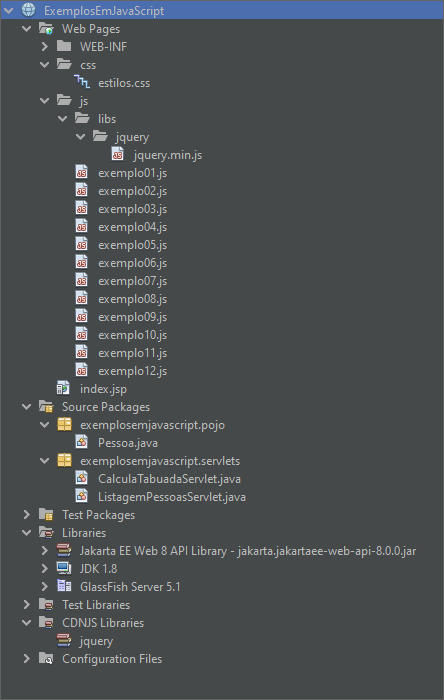
\includegraphics[scale=0.7]{imagens/cap07EstruturaDoProjeto}
    \\\textbf{Fonte:} Elaborada pelo autor
    \label{fig:cap07EstruturaDoProjeto}
\end{figure}
\FloatBarrier

Começaremos com o \texttt{index.jsp} apresentado na Listagem~\thechapter.\ref{listagem:projetos/capitulo07/ExemplosEmJavaScript/web/index.jsp}. Entre as linhas 10 e 22 usamos a \textit{tag} \inlineHTMLCode{<script>} para carregarmos no documento treze arquivos de código JavaScript. Inclusive, essa mesma \textit{tag} pode ser utilizada para inserir código JavaScript no próprio documento. Veremos isso mais adiante. Na linha 10 é carregada a biblioteca jQuery que há alguns anos atrás era absolutamente relevante, mas que hoje em dia tem caído em desuso visto a evolução do JavaScript. Ela será tratada no livro pela sua importância em software legado, por facilitar e padronizar algumas coisas e também, é claro, por preferência minha :D. No restante das linhas são associados os arquivos com os exemplos que aprenderemos. O restante do documento consiste na construção de uma interface com alguns componentes e \textit{tags} que serão manipulados pelo nosso código em JavaScript. 

Os cinco primeiros exemplos são relativos às construções principais da linguagem. Veja que da linha 30 à 34 temos um parágrafo (\textit{tag} \inlineHTMLCode{<p>}) com um botão dentro (\textit{tag} \inlineHTMLCode{<button>}) e que em seu evento \textit{click}, representado pelo atributo \texttt{onclick}, é registrado uma função tratadora/manipuladora/ouvinte de evento (\textit{event handler} ou \textit{event listener}). Para registrar uma função como tratadora de um determinado evento, basta inserir seu nome no valor do atributo \texttt{onclick} e adicionar, entre os parânteses da mesma, a palavra \texttt{event}. Esse \texttt{event} carregará o objeto do evento que será disparado pela \textit{tag} e ouvido pela função. Essa função precisa estar declarada e implementada em algum lugar. No nosso caso, estará no arquivo \texttt{exemplo01.js}, referenciado acima. Note que como o JavaScript é interpretado, para se poder usar algo, essa ``coisa'' precisa ter sido declarada antes ou as vezes ``vista'' pelo interpretador pela primeira vez, sendo que esse segundo comportamento pode gerar muitos problemas caso não seja entendido apropriadamente, mas veremos isso também. Resumindo, ao se clicar (\texttt{onclick}) nesse primeiro botão, afunção \inlineJavaScriptCode{executarExemplo01(event)} será invocada. Fácil não é? Existe uma infinidade de eventos permitidos para cada \textit{tag}, mas falaremos de alguns deles à medida que for necessário. CEsse padrão de um botão invocando uma função se repetirá em praticamente todos os exemplos. Os cinco primeiros têm a mesma estrutura.

Nos exemplos 06, 07 e 08 trataremos da manipulação das \textit{tags}, como dinamicamente inserir conteúdo nas mesmas ou ler/escrever dados em componentes de formulário. Esses exemplos estão dentro da seção ``Manipulação do DOM'', onde DOM significa \textit{Document Object Mode}l que nos bastidores é uma árvore composta de objetos que representam o resultado do \textit{parse} do arquivo HTML pelo navegador ou cliente. Usando JavaScript podemos mexer nessa árvore, alterando atributos dos nós, que na maioria das vezes representam as \textit{tags}, além de inserir e remover nós. Todas as modificações são replicadas automaticamente pelo navegador que entende que a árvore foi alterada e precisa ser redesenhada no processo de renderização do documento. Antigamente, quando isso era novidade há mais de 20 anos atrás, era chamado de ``HTML Dinâmico'' (\textit{Dynamic} HTML (DHTML)). Sim, estou ficando velho :D. Perceba que nesses exemplos, além dos botões temos \textit{divs} que serão usadas para mostrar o resultado de algum processamento, além de componentes de formulário e outros botões no exemplo 08.

No exemplo 09 falaremos um pouco de tratamento de eventos, como já comentei anteriormente. Nesse exemplo, na linha 171, temos a invocação da função\newline%
\inlineJavaScriptCode{registrarEventosExemplo09()} em que, programaticamente, faremos o registro dos ouvintes de eventos ao invés de usar os atributos prefixados com ``\texttt{on}'' das \textit{tags}.

No exemplo 10 trataremos do uso da \textit{tag} \inlineHTMLCode{<canvas>} usada para desenhar programaticamente, realizando uma simulação física de uma bolinha.

Nos dois últimos exemplos trataremos das requisições assíncronas e de intercâmbio de dados entre cliente e servidor.

\htmlCode{Página principal da aplicação\newline%
Arquivo: \texttt{/index.jsp}}{projetos/capitulo07/ExemplosEmJavaScript/web/index.jsp}

Caso queira, durante os testes de execução, comente trechos do código do \texttt{index.jsp} para que você não precise ficar rolando a página para chegar em alguma parte toda vez que for testar uma funcionalidade.

Na Listagem~\thechapter.\ref{listagem:projetos/capitulo07/ExemplosEmJavaScript/web/css/estilos.css} é apresentado o arquivo com as folhas de estilo usadas no \texttt{index.jsp}. O código já contém os comentários para você entender o que se trata cada coisa.

\cssCode{Folhas de estilo do projeto\newline%
Arquivo: \texttt{/index.jsp}}{projetos/capitulo07/ExemplosEmJavaScript/web/css/estilos.css}

\begin{saibaMais}
    Sobre CSS, consulte \url{https://developer.mozilla.org/en-US/docs/Web/CSS} e \url{https://developer.mozilla.org/en-US/docs/Web/CSS/Reference}.
\end{saibaMais}

Nas próximas três listagens serão mostrados os componentes do lado do servidor que utilizaremos para os dois últimos exemplos. Na Listagem~\thechapter.\ref{listagem:projetos/capitulo07/ExemplosEmJavaScript/src/java/exemplosemjavascript/pojo/Pessoa.java} definimos a classe \texttt{Pessoa}, um \textit{Plain Old Java Object} (POJO) ou \textit{Value Object} (VO) que é uma classe que utilizaremos para criar objetos para transportar dados.

\javaCode{Classe Pessoa\newline%
Arquivo: \texttt{exemplosemjavascript/pojo/Pessoa.java}}{projetos/capitulo07/ExemplosEmJavaScript/src/java/exemplosemjavascript/pojo/Pessoa.java}

Na Listagem~\thechapter.\ref{listagem:projetos/capitulo07/ExemplosEmJavaScript/src/java/exemplosemjavascript/servlets/CalculaTabuadaServlet.java} é apresentado o código do Servlet \texttt{CalculaTabuadaServlet}, mapeado em \texttt{/calcularTabuada} que recebe um valor inteiro e retorna o texto representando a ``tabuada'' do número processado. Esse retorno é gerado pelo próprio Servlet no seu fluxo de saída (linhas 41, 42 e 43), sendo que o objeto response é configurado para indicar ao cliente que o que está chegando é no formato de texto puro (linha 28).

\javaCode{Servlet de tabuada\newline%
Arquivo: \texttt{exemplosemjavascript/servlets/CalculaTabuadaServlet.java}}{projetos/capitulo07/ExemplosEmJavaScript/src/java/exemplosemjavascript/servlets/CalculaTabuadaServlet.java}

Por fim, na Listagem~\thechapter.\ref{listagem:projetos/capitulo07/ExemplosEmJavaScript/src/java/exemplosemjavascript/servlets/ListagemPessoasServlet.java} é apresentado o código do Servlet \texttt{ListagemPessoasServlet}, mapeado em \texttt{/listarPessoas} que indica ao cliente que os dados que serão retornados irão no formato JavaScript Object Notation\footnote{O formato JSON será tratado no exemplo 05. Por enquanto assuma que é uma forma de codificar os dados de um objeto em forma de texto.} (JSON) (linha 33). Nesse Servlet é criada uma lista de objetos do tipo \texttt{Pessoa}, baseada na quantidade recebida via requisição e essa lista é serializada em JSON usando a camada de \textit{bindind} JSON-B do Java/Jakarta EE. Na linha 35 é criado o objeto serializador e na linha 56 ele é usado, convertendo a lista com os objetos do tipo \texttt{Pessoa} em uma representação em texto, que no nosso caso é o JSON.

\javaCode{Servlet de listagem de pessoas usando JSON\newline%
Arquivo: \texttt{exemplosemjavascript/servlets/ListagemPessoasServlet.java}}{projetos/capitulo07/ExemplosEmJavaScript/src/java/exemplosemjavascript/servlets/ListagemPessoasServlet.java}

Agora que temos toda a infraestrutura básica do nosso projeto, podemos começar a falar sobre JavaScript. Vamos começar!



\section{Funções de E/S e Operadores Aritméticos}

Começaremos nossa breve jornada de descoberta da linguagem JavaScript aprendendo uma forma de obter dados do usuário, que normalmente não é usada em um software em produção, mas para aprender conceitos vai nos servir no momento, como gerar saída, declarar variáveis e realizar as operações aritméticas básicas. Na Listagem~\thechapter.\ref{listagem:projetos/capitulo07/ExemplosEmJavaScript/web/js/exemplo01.js} pode ser visto o código completo do primeiro exemplo. Veja que logo na primeira linha há a declaração da função \inlineJavaScriptCode{executarExemplo01(event)} que é a função que tratará o evento \texttt{click} do primeiro botão do \texttt{index.jsp}.

\javaScriptCode{Exemplo 01\newline%
Arquivo: \texttt{/js/exemplo01.js}}{projetos/capitulo07/ExemplosEmJavaScript/web/js/exemplo01.js}

Na linha 5 é declarada uma variável local usando a palavra chave \inlineJavaScriptCode{let}\footnote{Veremos o propósito da palavra chave \texttt{let} no exemplo 02.}, com o identificador \inlineJavaScriptCode{n1} e atribuímos a ela o retorno da função \inlineJavaScriptCode{prompt}. Essa função recebe como parâmetro uma String que, ao ser executada, apresenta ao usuário um diálogo com uma mensagem -vinda da String passada- um campo de texto, um botão de confirmação e um de cancelamento. Ao se clicar no botão de confirmação o valor fornecido do campo de texto será retornado ao chamador, no caso, atribuído à variável \inlineJavaScriptCode{n1} e se o diálogo for cancelado, será retornado o valor \inlineJavaScriptCode{null}. O retorno é do tipo String. Note que não declaramos o tipo das variáveis em JavaScript, pois a tipagem das variáveis é dinâmica, visto que o tipo de cada variável depende do valor atribuído ou referenciado por ela.

Na linha 9 fazemos basicamente a mesma coisa para a variável \inlineJavaScriptCode{n2}, mas o retorno da função \inlineJavaScriptCode{prompt} é usada como argumento da função \inlineJavaScriptCode{Number} que converterá a String retornada por \inlineJavaScriptCode{prompt} em um número e então esse valor será atribuído a \inlineJavaScriptCode{n2}.

Entre as linhas 12 e 16 declaramos cinco novas variáveis e atribuímos a elas o resultado de cinco operações. Note que como \inlineJavaScriptCode{n1} referencia uma String, o operador \inlineJavaScriptCode{+} será tratado como operador de concatenação de Strings ao invés de adição, ou seja, \inlineJavaScriptCode{n2} será convertida para String e concatenada com \inlineJavaScriptCode{n1}! Os outros operadores como são aplicáveis apenas à números, \inlineJavaScriptCode{n1} será convertido implicitamente e a operação será realizada. O resultado disso será visto na saída que será gerada e exibida.

Falando da saída, na linha 19 declaramos a variável \inlineJavaScriptCode{saida} e concatenamos diversas Strings para gerar o resultado. Em JavaScript existem três literais para Strings:
  
\begin{enumerate}
    \item Delimitadas por aspas simples (apóstrofo): \inlineJavaScriptCode{'uma string'};
    \item Delimitadas por aspas duplas (aspas): \inlineJavaScriptCode{"outra string"};
    \item Delimitadas por acento grave (crase): \inlineJavaScriptCode{`mais uma string`};
\end{enumerate}

Os dois primeiros são análogos, com a diferença que quando se usa aspas simples como delimitador e queremos ter uma aspas simples dentro da String, precisamos escapá-la com contrabarra (barra invertida) e as aspas duplas não precisam. Por exemplo, \inlineJavaScriptCode{'a\'b"c'} corresponde à \destaque{\texttt{a\textquotesingle{}b"c}}. Quando delimitamos a String com aspas duplas temos o contrário, ou seja, \inlineJavaScriptCode{"a'b\"c"} correspondendo à \destaque{\texttt{a\textquotesingle{}b"c}}.

O terceiro tipo de delimitador é mais interessante, pois permite que façamos a interpolação de valores dentro da String usando uma notação parecida com a da EL do Java Web, mas que não tem relação a não ser a sintaxe similar. Para o nosso exemplo, se \inlineJavaScriptCode{n1} valer \inlineJavaScriptCode{"10"} e \inlineJavaScriptCode{n2} valer \inlineJavaScriptCode{5}, o resultado de \inlineJavaScriptCode{`${n1} e ${n2}`} será \destaque{\texttt{10 e 5}}.

Por fim, para apresentar a String gerada, usamos duas formas. A primeira, na linha 29, com a função \inlineJavaScriptCode{alert} que, assim como \inlineJavaScriptCode{prompt}, é bloqueante, fazendo a execução do código parar naquele ponto ao esperar a interação do usuário. Essa função recebe uma String como parâmetro e a mostra num diálogo ao ser executada. A outra forma é usando a função \inlineJavaScriptCode{log} do objeto \inlineJavaScriptCode{console}, que recebe um objeto como parâmetro e o mostra no console do navegador. No nosso exemplo, a exibição no console está condicionada ao retorno da função \inlineJavaScriptCode{confirm} que exibe uma mensagem ao usuário e aguarda a interação. Caso o usuário confirme a mensagem, a função retornará um valor verdadeiro, usado na estrutura condicional \inlineJavaScriptCode{if} do exemplo.



\section{Declarações de Variáveis e Suas Implicações}

Nesta seção trataremos as variáveis e as declarações delas em JavaScript. Como já dito, as variáveis não tem um tipo definido, visto que a linguagem é dinamicamente tipada, implicando que o tipo da variável varia de acordo com o que ela referencia. Em JavaScript temos Strings, números, valores lógicos, funções, objetos entre outros.

Toda variável em JavaScript ao ser declarada passará pelo processo de \textit{hoisting}. Nesse processo, a variável será elevada ou içada até o início ou topo do contexto em que ela foi declarada e que passará a existir. A ideia é que quando o interpretador encontra uma declaração de variável e ela é bem sucedida, ou seja, é sintática e semanticamente correta, ela passará a existir como se houvesse sido declarada no início do escopo em que reside.

Podemeos influenciar em como esse içamento ocorrerá em relação à inicialização das variáveis. Veja a lista abaixo, temos quatro formas de declarar variáveis:

\begin{enumerate}
    \item \inlineJavaScriptCode{let variavel = "valor";};
    \item \inlineJavaScriptCode{var variavel = "valor";};
    \item \inlineJavaScriptCode{variavel = "valor";};
    \item \inlineJavaScriptCode{const constante = "valor";};
\end{enumerate}

Quando a palavra-chave \inlineJavaScriptCode{let} é usada, a variável só poderá ser usada depois da sua inicialização, mesmo havendo \textit{hoisting} para sua declaração. O mesmo acontece com as constantes, declaradas com \inlineJavaScriptCode{const}. Já as variáveis declaradas com a palavra-chave \inlineJavaScriptCode{var} serão inicializadas com \inlineJavaScriptCode{undefined}. Por fim, as variáveis que são declaradas sem indicar nenhuma dessas três palavras-chave passarão a existir no escopo global, o que pode trazer uma série de problemas. Imagine que você declarou mais de uma variável com o mesmo nome em dois ou mais escopos diferentes. A declaração de fato ocorrerá quando o interpretador a encontrar pela primeira vez e, independende de onde for, ela passará a existir no escopo global e a partir desse ponto você pode perder o controle do valor que a variável referencia se não tomar muito cuidado com o que está fazendo. O ideal é não utilizar ok?

O exemplo apresentado na Listagem~\thechapter.\ref{listagem:projetos/capitulo07/ExemplosEmJavaScript/web/js/exemplo02.js} mostra todos esses efeitos quando for executado. O ``problema'' da variável declarada sem \inlineJavaScriptCode{let}, \inlineJavaScriptCode{var} ou \inlineJavaScriptCode{const} pode ser reproduzido ao se clicar pela segunda vez no botão do exemplo 02.

\javaScriptCode{Exemplo 02\newline%
Arquivo: \texttt{/js/exemplo02.js}}{projetos/capitulo07/ExemplosEmJavaScript/web/js/exemplo02.js}

Veja o exemplo, todo o código está comentado, não sendo necessário entrar em mais detalhes. Recomendo que você dê uma olhada nos \textit{links} disponibilizados nas próximas duas caixas ``Saiba Mais''.

\begin{saibaMais}
    Para uma explicação mais detalhada sobre essas implicações, acesse \url{http://www.constletvar.com/}.
\end{saibaMais}

\begin{saibaMais}
    Para mais detalhes sobre variáveis de clarações em JavaScript, acesse \url{https://developer.mozilla.org/en-US/docs/Web/JavaScript/Reference/Statements}.
\end{saibaMais}

Esse conceito pode gerar muita confusão, inclusive se declararmos uma variável com \inlineJavaScriptCode{var} no contexto global (fora de funções) ela será uma variável global (uma propriedade do objeto \texttt{window}), ao passo que dentro de uma função ela terá escopo local, assim como \inlineJavaScriptCode{let} e \inlineJavaScriptCode{const}, mas inicializada como \inlineJavaScriptCode{undefined}. Ainda, é importante frisar que uma constante tem ligação imutável (\textit{immutable binding}) com o que ela referencia, ou seja, ela não pode receber um novo valor, mas o valor que ela referencia pode ser modificado (ela não é imutável), por exemplo, se for um objeto e quisermos alterar alguma de suas propriedades.



\section{Estruturas Condicionais e Operadores}

Em JavaScript temos as mesmas estruturas condicionais presentes na maioria das linguagens de programação ou seja, um \inlineJavaScriptCode{if} com \inlineJavaScriptCode{else} aninhados e opcionais e um \inlineJavaScriptCode{switch}. Os operadores relacionais e lógicos também são os operadores padrão encontrados na maioria das linguages derivadas de C, com a adição de mais dois operadores relacionais que são o operador de identidade (\inlineJavaScriptCode{===}) e o operador de não identidade (\inlineJavaScriptCode{!==}). Ao passo que os operadores de igualdade e de desigualdade verificam se o valor dos operandos comparados são respectivamente iguais ou difentes, inclusive após a conversão implícita de algum deles, os operadores de identidade e de não identidade verificam, além do valor, agora sem conversão implícita, se, respectivamente, o tipo é o mesmo ou se é diferente. Na Listagem~\thechapter.\ref{listagem:projetos/capitulo07/ExemplosEmJavaScript/web/js/exemplo03.js} pode ser visto o emprego das estruturas condicionais e a declaração de variáveis com alguns valores permitidos.

\javaScriptCode{Exemplo 03\newline%
Arquivo: \texttt{/js/exemplo03.js}}{projetos/capitulo07/ExemplosEmJavaScript/web/js/exemplo03.js}

\begin{saibaMais}
    Para mais detalhes sobre os operadores em JavaScript, acesse \url{https://developer.mozilla.org/en-US/docs/Web/JavaScript/Reference/Operators}.
\end{saibaMais}


\section{Estruturas de Repetição e Arrays}

Texto.

Listagem~\thechapter.\ref{listagem:projetos/capitulo07/ExemplosEmJavaScript/web/js/exemplo04.js}

\javaScriptCode{Exemplo 04\newline%
Arquivo: \texttt{/js/exemplo04.js}}{projetos/capitulo07/ExemplosEmJavaScript/web/js/exemplo04.js}

\begin{saibaMais}
    Para mais detalhes sobre o tipo Array em JavaScript, acesse \url{https://developer.mozilla.org/en-US/docs/Web/JavaScript/Reference/Global_Objects/Array}.
\end{saibaMais}

\section{``Classes'', Objetos e JSON}

Texto.

Listagem~\thechapter.\ref{listagem:projetos/capitulo07/ExemplosEmJavaScript/web/js/exemplo05.js}

\javaScriptCode{Exemplo 05\newline%
Arquivo: \texttt{/js/exemplo05.js}}{projetos/capitulo07/ExemplosEmJavaScript/web/js/exemplo05.js}

\begin{saibaMais}
    Para saber mais sobre classes em JavaScript, acesse \url{https://developer.mozilla.org/en-US/docs/Web/JavaScript/Reference/Classes}.
\end{saibaMais}

\begin{saibaMais}
    Para consultar a documentação sobre o tipo String em JavaScript, acesse \url{https://developer.mozilla.org/en-US/docs/Web/JavaScript/Reference/Global_Objects/String}.
\end{saibaMais}

\begin{saibaMais}
    Para consultar a documentação sobre JSON em JavaScript, acesse \url{https://developer.mozilla.org/en-US/docs/Web/JavaScript/Reference/Global_Objects/JSON}.
\end{saibaMais}


\section{Manipulação do DOM}

Texto. Lembrar do termo DHTML (não se usa mais!).

\begin{saibaMais}
    A documentação do DOM pode ser vista no \textit{link} \url{https://developer.mozilla.org/en-US/docs/Web/API/Document_Object_Model}.
\end{saibaMais}

\subsection{JavaScript Puro}

Texto.

Listagem~\thechapter.\ref{listagem:projetos/capitulo07/ExemplosEmJavaScript/web/js/exemplo06.js}

\javaScriptCode{Exemplo 06\newline%
Arquivo: \texttt{/js/exemplo06.js}}{projetos/capitulo07/ExemplosEmJavaScript/web/js/exemplo06.js}


\subsection{Usando jQuery}

A biblioteca jQuery\footnote{\url{https://jquery.com/}}...

Listagem~\thechapter.\ref{listagem:projetos/capitulo07/ExemplosEmJavaScript/web/js/exemplo07.js}

\javaScriptCode{Exemplo 07\newline%
Arquivo: \texttt{/js/exemplo07.js}}{projetos/capitulo07/ExemplosEmJavaScript/web/js/exemplo07.js}

\begin{saibaMais}
    Se quiser aprender um pouco mais sobre a jQuery, acesse \url{https://learn.jquery.com/}.
\end{saibaMais}


\section{Manipulação de Formulários}

Texto.

Listagem~\thechapter.\ref{listagem:projetos/capitulo07/ExemplosEmJavaScript/web/js/exemplo08.js}

\javaScriptCode{Exemplo 08\newline%
Arquivo: \texttt{/js/exemplo08.js}}{projetos/capitulo07/ExemplosEmJavaScript/web/js/exemplo08.js}


\section{Eventos}

Texto.

Listagem~\thechapter.\ref{listagem:projetos/capitulo07/ExemplosEmJavaScript/web/js/exemplo09.js}

\javaScriptCode{Exemplo 09\newline%
Arquivo: \texttt{/js/exemplo09.js}}{projetos/capitulo07/ExemplosEmJavaScript/web/js/exemplo09.js}

\begin{saibaMais}
    A documentação completa sobre os eventos que podem ser tratados pode ser vista em  \url{https://developer.mozilla.org/en-US/docs/Web/Events}.
\end{saibaMais}



\section{Simulação Usando \textit{Canvas}}

Texto.

Listagem~\thechapter.\ref{listagem:projetos/capitulo07/ExemplosEmJavaScript/web/js/exemplo10.js}

\javaScriptCode{Exemplo 10\newline%
Arquivo: \texttt{/js/exemplo10.js}}{projetos/capitulo07/ExemplosEmJavaScript/web/js/exemplo10.js}

\begin{saibaMais}
    A API do Canvas pode ser vista em \url{https://developer.mozilla.org/en-US/docs/Web/API/Canvas_API}.
\end{saibaMais}



\section{Requisições Assíncronas e Intercâmbio de Dados}

Texto. Falar da Web Worker API

\begin{saibaMais}
    Mais sobre a API Web Workers \url{https://developer.mozilla.org/en-US/docs/Web/API/Web_Workers_APII}.
\end{saibaMais}


\subsection{AJAX com jQuery e com Fetch API}

Texto.

Listagem~\thechapter.\ref{listagem:projetos/capitulo07/ExemplosEmJavaScript/web/js/exemplo11.js}

\javaScriptCode{Exemplo 11\newline%
Arquivo: \texttt{/js/exemplo11.js}}{projetos/capitulo07/ExemplosEmJavaScript/web/js/exemplo11.js}

\begin{saibaMais}
    Documentação da função jQuery.ajax(): \url{https://api.jquery.com/jquery.ajax/}.
\end{saibaMais}

\begin{saibaMais}
    Documentação da Fetch API: \url{https://developer.mozilla.org/en-US/docs/Web/API/Fetch_API}.
\end{saibaMais}


\subsection{AJAX jQuery e com Fetch API Processando JSON}

Texto.

\url{https://developer.mozilla.org/en-US/docs/Web/API/Fetch_API/Using_Fetch}

Listagem~\thechapter.\ref{listagem:projetos/capitulo07/ExemplosEmJavaScript/web/js/exemplo12.js}

\javaScriptCode{Exemplo 12\newline%
Arquivo: \texttt{/js/exemplo12.js}}{projetos/capitulo07/ExemplosEmJavaScript/web/js/exemplo12.js}


\section{Resumo}


\section{Exercícios}


\section{Projetos}
